%----------------------------------------------------------------------------------------
%    PACKAGES AND THEMES
%----------------------------------------------------------------------------------------

\documentclass[aspectratio=169,xcolor=dvipsnames]{beamer}
\usetheme{SimpleDarkBlue}
\setbeamertemplate{blocks}[rounded]

\usepackage{hyperref}
\usepackage{graphicx} % Allows including images
\usepackage{booktabs} % Allows the use of \toprule, \midrule and \bottomrule in tables
\usepackage{algorithm2e}
\definecolor{lightred}{RGB}{255, 182, 193}
\definecolor{lightgreen}{RGB}{144, 238, 144}

%----------------------------------------------------------------------------------------
%    TITLE PAGE
%----------------------------------------------------------------------------------------

\title{Multi Agent Reinforcement Learning (MARL)}

\author{Adam Lagssaibi, Dabier Edgard, Nolan Sisouphanthong\\
    \small \textbf{Supervisor}: Alexandre Reiffers-Masson}

\institute
{
    Project on recent advance in machine learning \\
    IMT Atlantique
}
\date{March 28, 2025} % Date, can be changed to a custom date

%----------------------------------------------------------------------------------------
%    PRESENTATION SLIDES
%----------------------------------------------------------------------------------------

\begin{document}

\begin{frame}
    % Print the title page as the first slide
    \titlepage
\end{frame}

%------------------------------------------------

\begin{frame}{Overview}
    \tableofcontents
\end{frame}

%------------------------------------------------
\section{Introduction to Reinforcement Learning (RL)}

\begin{frame}[plain]
    \vspace{0.15\textheight}
    \begin{center}
        {\bfseries Section \thesection} 
        
        \vspace{0.5cm} 
        
        {\Large\bfseries\insertsectionhead} 
    \end{center}
\end{frame}
%------------------------------------------------

\begin{frame}{What is Reinforcement Learning?}
    RL is part of Machine Learning, but is neither supervised or unsupervised learning.
    \begin{figure}[h]
    \centering
    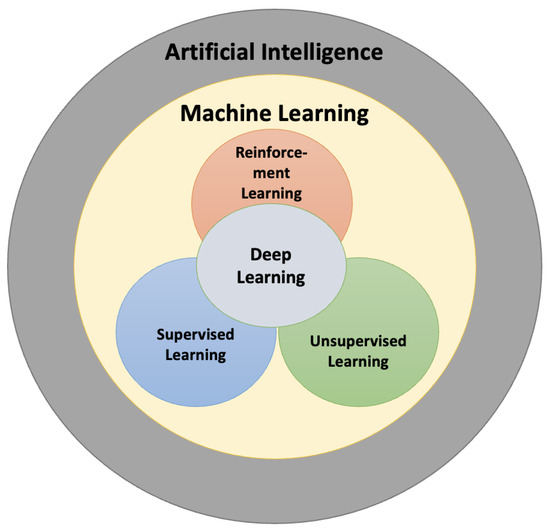
\includegraphics[scale=0.35]{images/RL_in_ML.jpg}
    \caption{Reinforcement Learning inside Machine Learning\textsuperscript{1}}
    \end{figure}
    \vspace{-5pt}
    \footnotesize \tiny \textsuperscript{1} Fahad Mon et al., \textit{Reinforcement Learning in Education: A Literature Review}, 2023. \url{https://www.mdpi.com/2227-9709/10/3/74}
\end{frame}

%------------------------------------------------

\begin{frame}{The FrozenLake example}

    \centering
    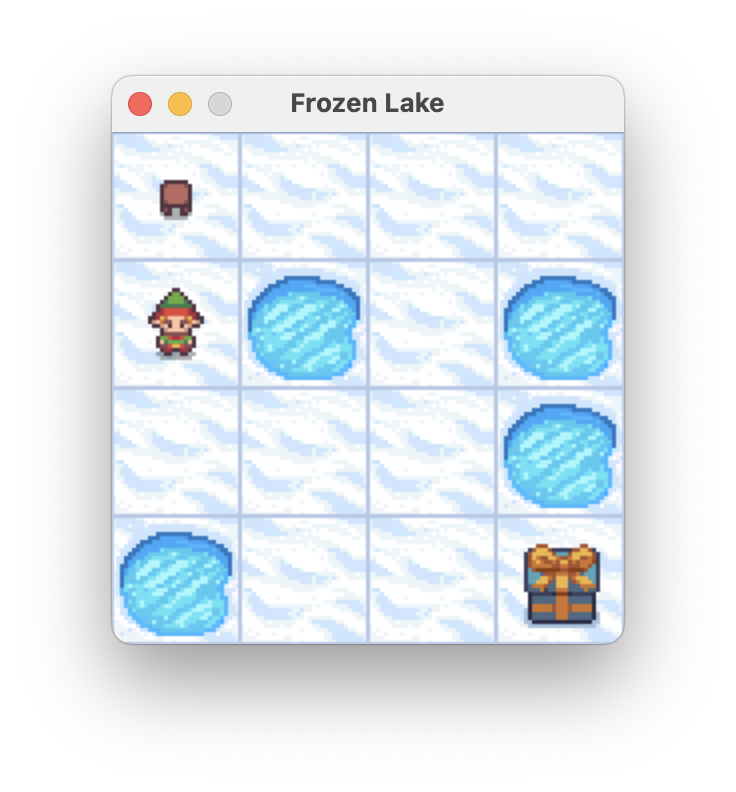
\includegraphics[scale=0.6]{images/single-agent.png}

\end{frame}

%------------------------------------------------

\begin{frame}{The FrozenLake example}

The \textbf{environment} of the game is made of ice path, holes, and a goal to be reached by the agent.
    
    \centering
    \begin{wrapfigure}{\textwidth}
        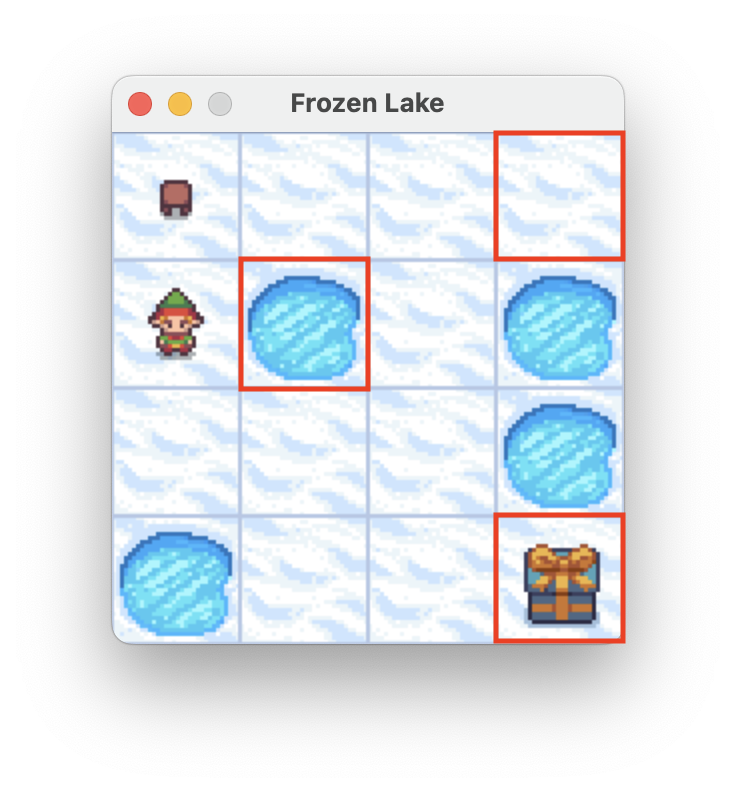
\includegraphics[scale=0.5]{images/env-elements.png}
    \end{wrapfigure}

\end{frame}

%------------------------------------------------

\begin{frame}{The FrozenLake example}

The agent can move around over time in the environment, we call this its \framebox{\textbf{actions} $\textbf{a}$}, such that he is in a \framebox{\textbf{state} $\textbf{s}$} at \framebox{time $\textbf{t}$}.

\centering
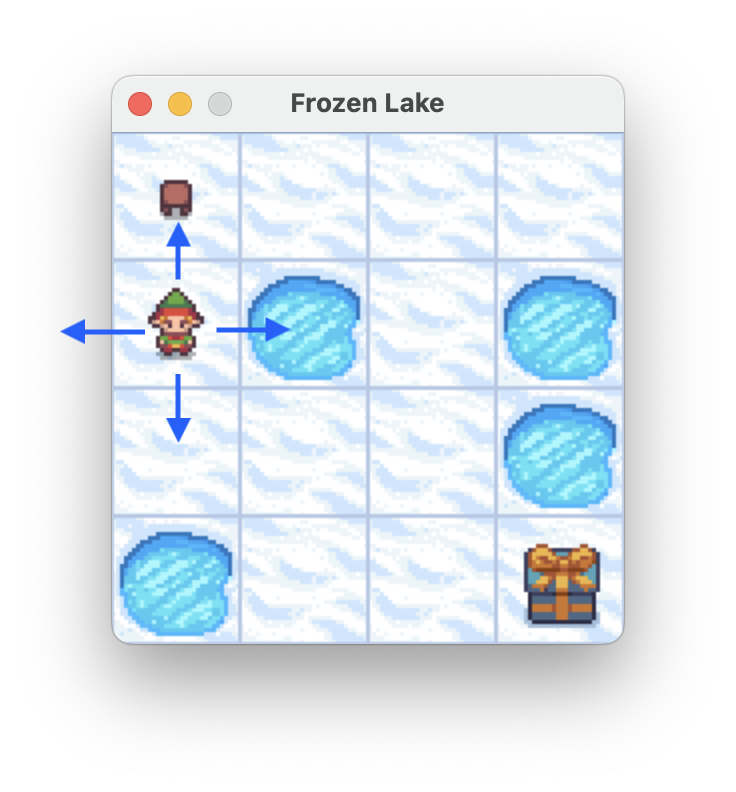
\includegraphics[scale=0.5]{images/moving-agent.png}

\end{frame}

%------------------------------------------------

\begin{frame}{The FrozenLake example}

Depending on the agent's actions, he can end up \underline{falling} in a hole or \underline{reaching} the goal.
    
\begin{figure}[h!]
    \centering
    \begin{minipage}{0.45\textwidth} 
        \centering
        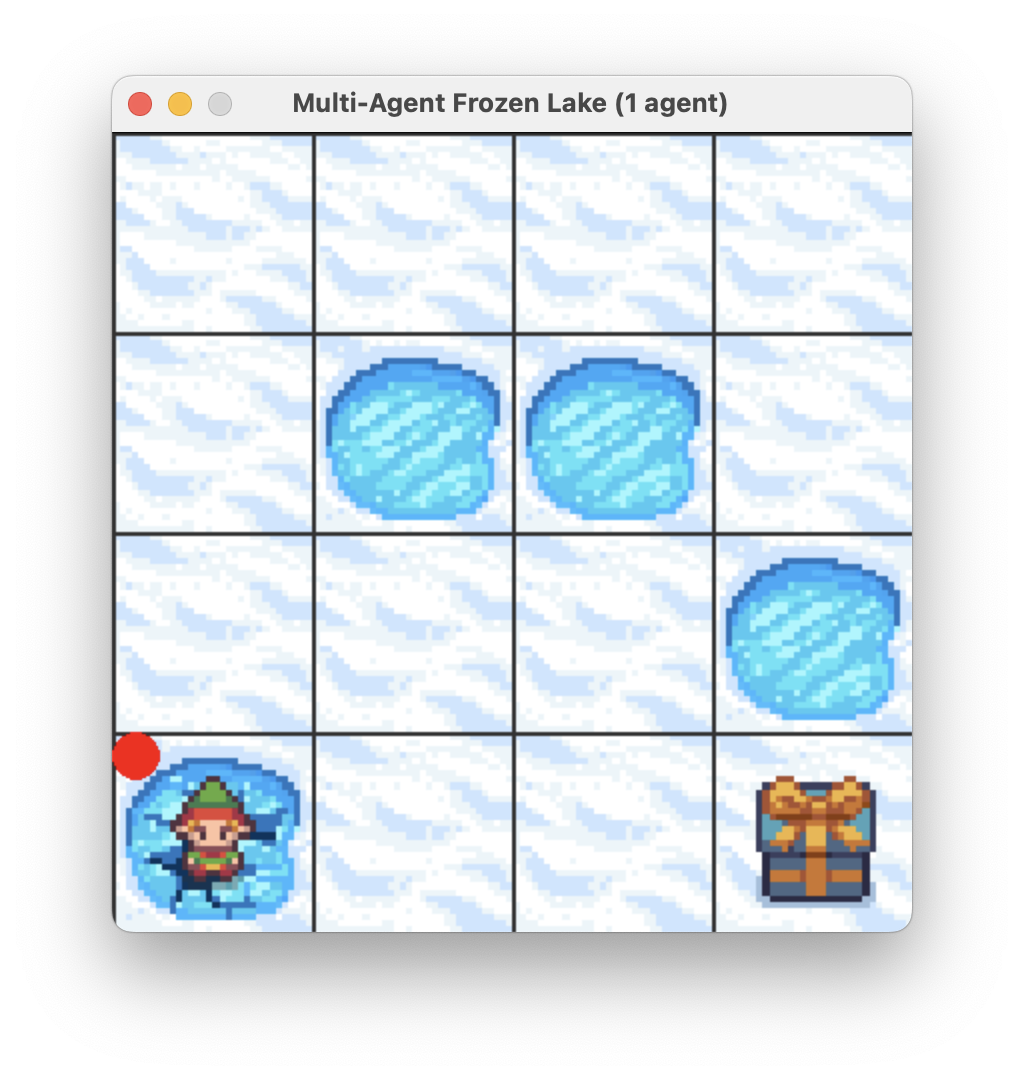
\includegraphics[scale=0.3]{images/fallen-agent.png}
        \caption{Fallen Agent}
    \end{minipage}%
    \begin{minipage}{0.45\textwidth} 
        \centering
        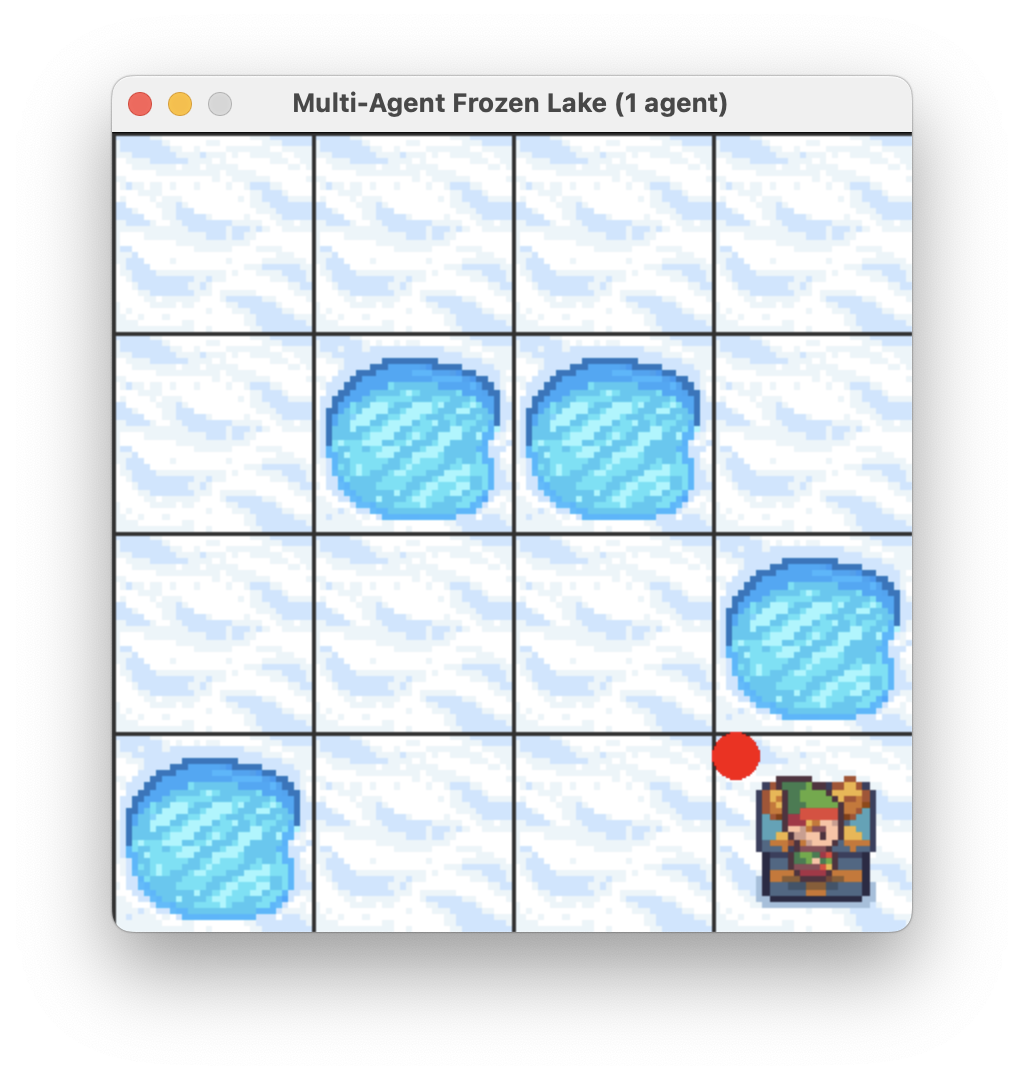
\includegraphics[scale=0.3]{images/goal-agent.png}
        \caption{Goal Agent}
    \end{minipage}
\end{figure}

\end{frame}

%------------------------------------------------

\begin{frame}{Markovianity property}

\begin{block}{Key notion : \textbf{Markovianity} of the action chain}
The probability of the agent being in a new state and receiving some reward only depends on its previous state and what action it takes, but not all the previous actions.
\vspace{10pt}

\centering
$P(s^{t+1} | s^t, a^t, s^{t-1}, a^{t-1}, ..., s^0, a^0) = P(s^{t+1} | s^t, a^t)$

\end{block}
\begin{center}
    \begin{minipage}{0.4\textwidth} 
        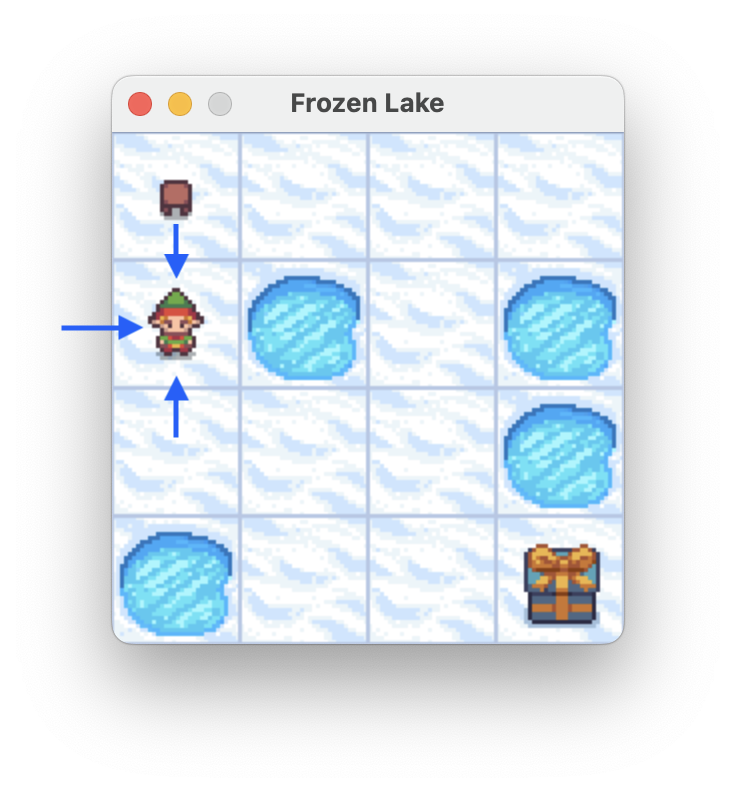
\includegraphics[scale=0.4]{images/previous-move.png}
    \end{minipage}
    \begin{minipage}{0.55\textwidth}
        The agent has to \textbf{learn} what actions to take when at a certain state.
        
        \vspace{10pt}
        This is called its \framebox{ \textbf{policy, $\pi$ }}.
        \vspace{10pt}
         \[
\pi: S \rightarrow A
\]
   
    \end{minipage}
\end{center}
\end{frame}

%------------------------------------------------

\begin{frame}{What is a good action?}
    We define a  \framebox{\textbf{reward function} \textbf{\emph{r}}} to indicate the agent if his action has a positive or negative impact on the objective.

    \begin{figure}[h!]
        \centering
        \begin{minipage}{0.45\textwidth} 
            \centering
            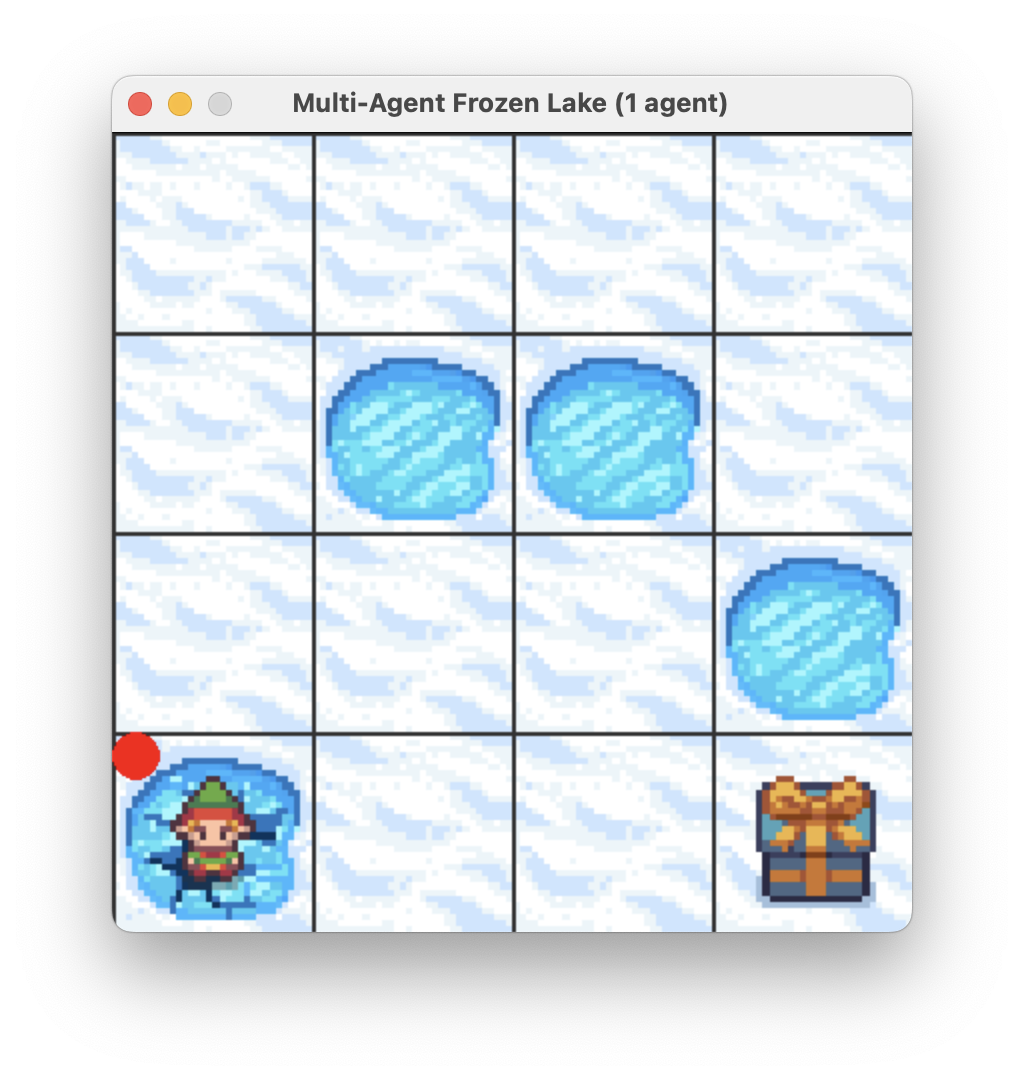
\includegraphics[scale=0.3]{images/fallen-agent.png}
            \caption{Reward = \textbf{-1}}
        \end{minipage}%
        \begin{minipage}{0.45\textwidth} 
            \centering
            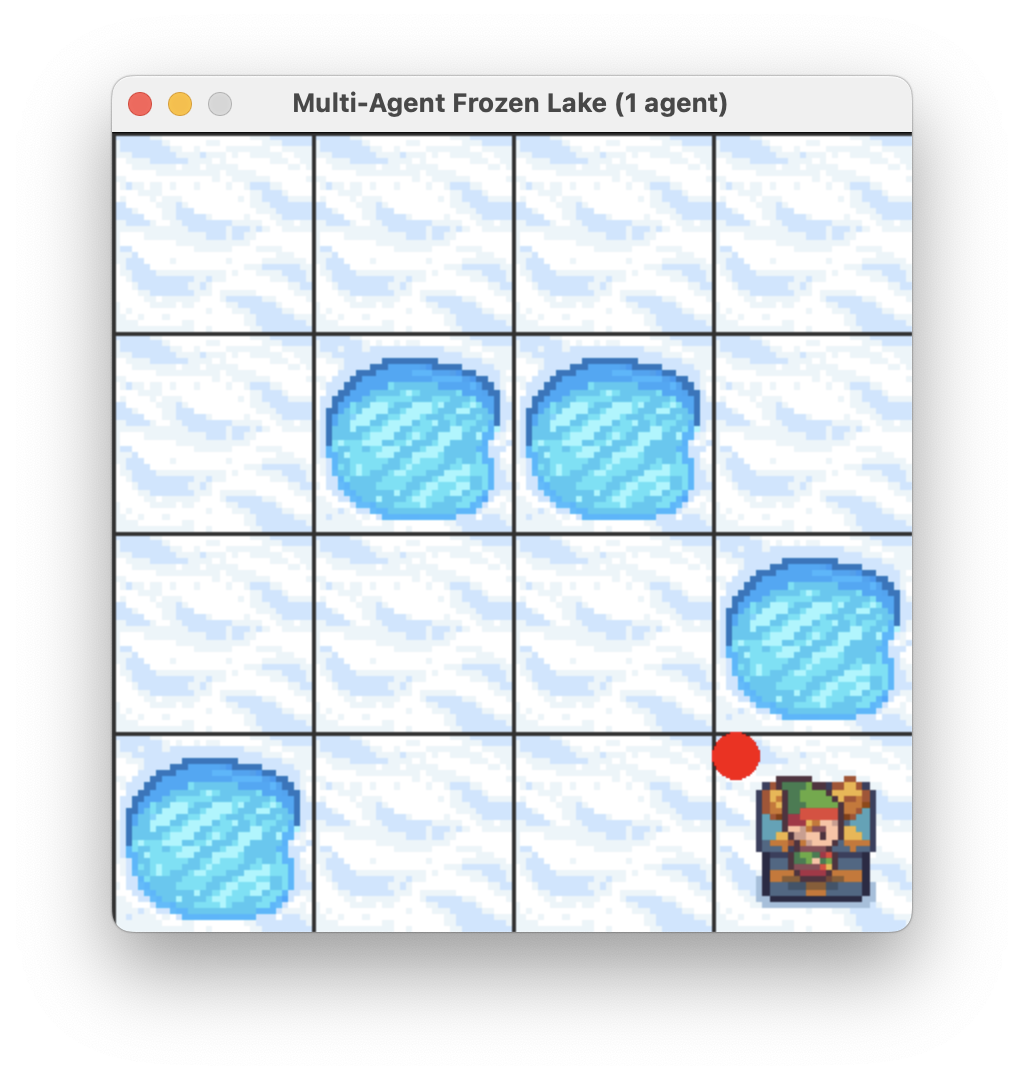
\includegraphics[scale=0.3]{images/goal-agent.png}
            \caption{Reward = \textbf{+1}}
        \end{minipage}
    \end{figure}
    
\end{frame}

%------------------------------------------------

\begin{frame}{Episodes and total return}

\begin{block}{Ending a run}
    We have to set limits so the agent doesn't run forever. We define
\vspace{10pt}
\begin{itemize}
    \item \underline{final states}: if the agent reaches them, we finish
    \item \underline{maximum time steps}: the amount of authorized steps for the agent
\end{itemize}
\vspace{10pt}
Once a final state is reached or the agent exceeds the maximum time step, the game is over. We call this entire process an \framebox{\textbf{episode}}.

\vspace{10pt}

At the end of an episode, we cumulate all the agent's rewards in the \framebox{\textbf{total return}}.

$r = \sum_{i=0}^T r^i$
\end{block}

\end{frame}

%------------------------------------------------

\begin{frame}{Summary}

\begin{minipage}{0.8\textwidth} 
    \vspace{-10pt}
    \begin{itemize}
        \item \textbf{Actions:} The agent can take \underline{actions}: $a$
        \vspace{10pt}
        
        \item \textbf{Reward:} The agent gets \underline{rewards} depending on its action: $r$
        \vspace{10pt}
        
        \item \textbf{Objective - episodes:} When reaching the \underline{goal}, or exceeding the \underline{maximum time step}, we end the \underline{episode}
        \vspace{10pt}

        \item \textbf{policy:} The agent learns a policy $\pi$ telling him what action $a$ to take on any given state $s$
        \vspace{10pt}

        \item \textbf{Total return:} At the end of an episode, we add up all the rewards in the \underline{total reward}: $r = \sum_{i=0}^T r^i$
    \end{itemize}
\end{minipage}%
\hspace{0.01\textwidth}
\begin{minipage}{0.1\textwidth} 
    \hspace{-9pt}
    \begin{minipage}{\textwidth}
        \centering
        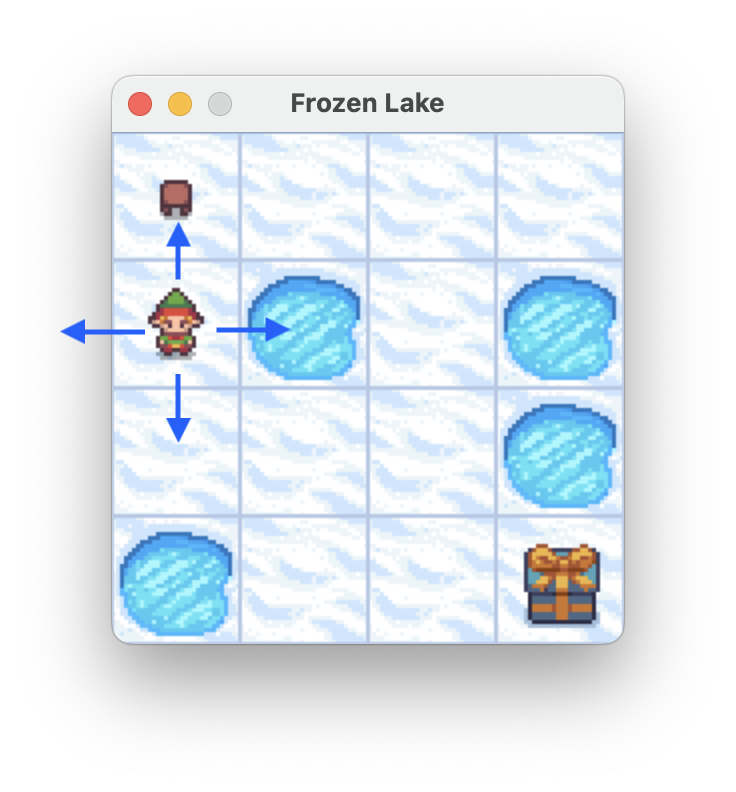
\includegraphics[scale=0.23]{images/moving-agent.png}
    \end{minipage}
    \vspace{-20pt}
    \vfill % Ensures the next image will be placed below the first
    \begin{minipage}{\textwidth}
        \centering
        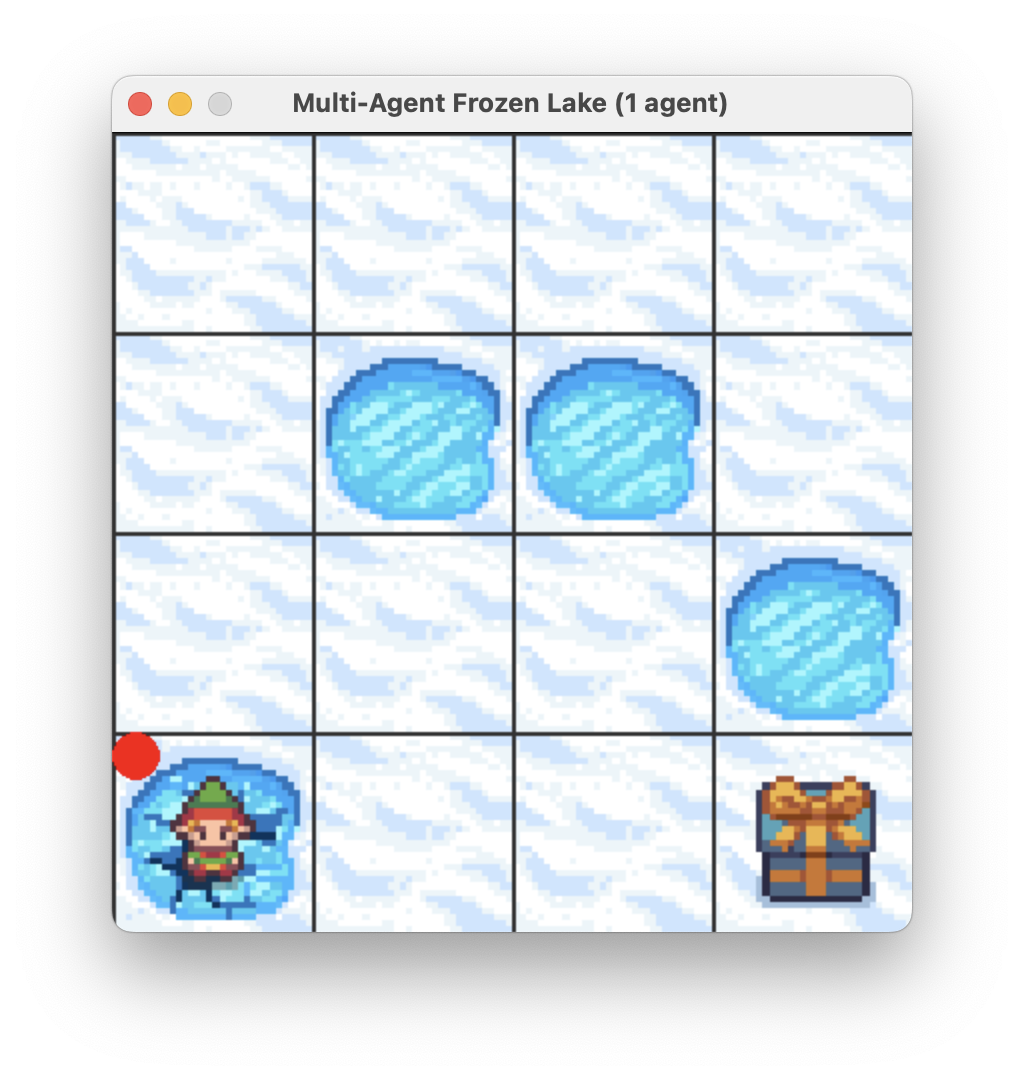
\includegraphics[scale=0.15]{images/fallen-agent.png}
    \end{minipage}
    \vspace{-15pt}
    \vfill
    \begin{minipage}{\textwidth}
        \centering
        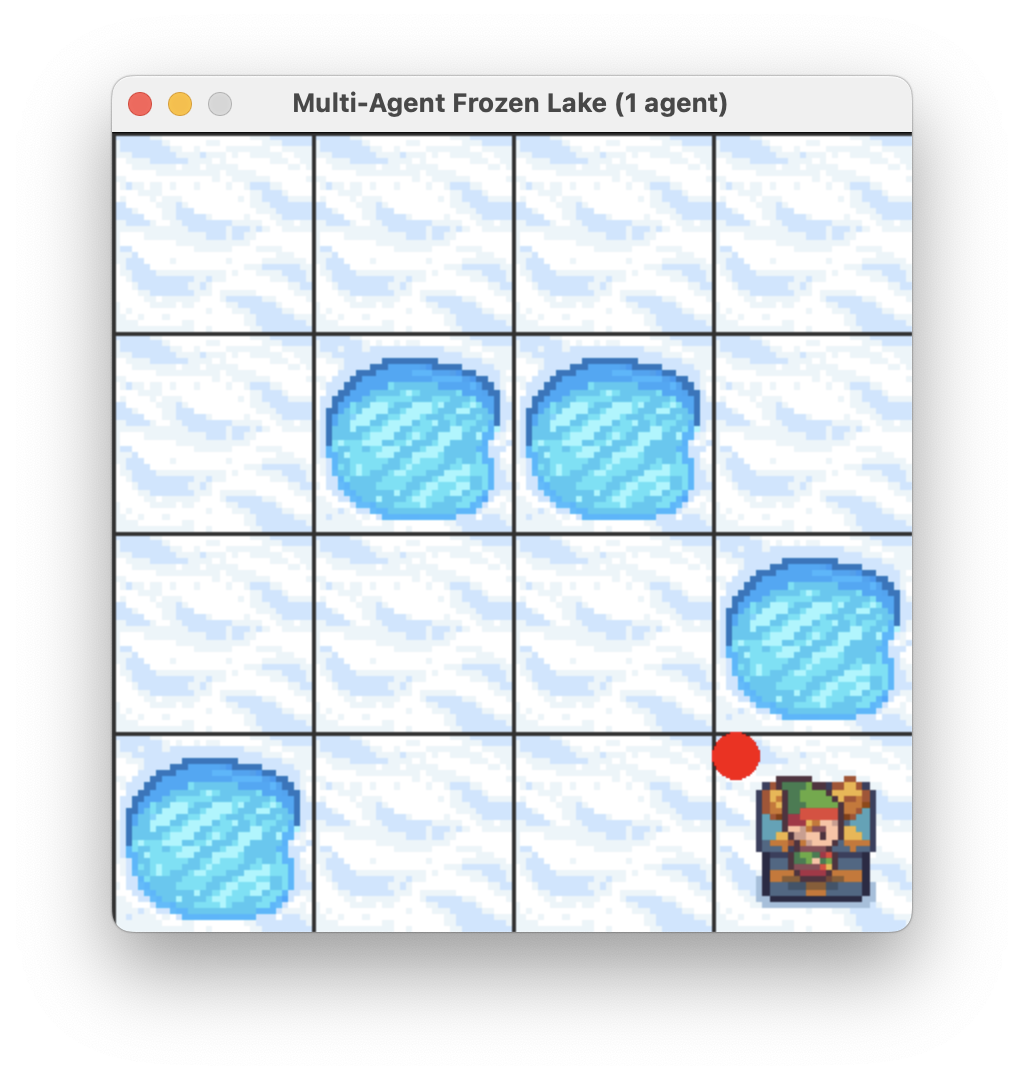
\includegraphics[scale=0.15]{images/goal-agent.png}
    \end{minipage}
\end{minipage}

\end{frame}

%------------------------------------------------

\begin{frame}{Discount factor}

\begin{block}{Reward design}    
    The reward choice shapes what the agent will learn
    \vspace{10pt}
    \begin{itemize}
        \item Direct cumulative reward for long term objectives
        \item Discounted reward to favor reaching the objective faster (greedy action taking):
    \end{itemize}
        \vspace{10pt}
        We introduce the \framebox{\textbf{discount factor $\gamma \in [0,1]$}} such that we favor the first moves
        \vspace{10pt}
\end{block}
        
\centering
$ r = \displaystyle \sum_{i=0}^T \gamma^i * r^i \to $ the agent learns to reach the goal faster 


\end{frame}

%------------------------------------------------

\begin{frame}{Dealing with Uncertainty in Games}

    \begin{block}{What is Uncertainty?}
    
        Recall the markovian property: $P(s^{t+1} | s^t, a^t, s^{t-1}, a^{t-1}, ..., s^0, a^0) = P(s^{t+1} | s^t, a^t)$
    
        \vspace{10pt}
        In some games, things don’t always go as planned.  
        \vspace{10pt}
        \begin{itemize}
            \item In a \framebox{\textbf{slippery game}}, the agent might slip and not move where it wants to.
            \item Some plans are riskier than others.
        \end{itemize}
        \vspace{10pt}
        We need to find the best plan that gets the most rewards, even with uncertainty.  
        \vspace{10pt}
    \end{block}
    
    \centering
    To pick the best plan, we test it many times and calculate the average reward: \\
    $ \text{Average Reward} = $E(r) = E_{\pi} \left[\displaystyle\sum_{i=0}^T \gamma^i \times r^i\right]

\end{frame}

%------------------------------------------------

\begin{frame}{Value Functions}

\begin{block}{What Are Value Functions?}
    Value functions help the agent know how good a situation is in the game $\to$ learn the optimal policy. 
    \begin{itemize}
        \item \framebox{\textbf{State-Value Function $V^\pi(s)$}}: How much reward the agent expects to get starting from a spot $s$ (a state) if it follows a plan $\pi$.
        \item \framebox{\textbf{Action-Value Function $Q^\pi(s, a)$}}: How much reward the agent expects to get if it takes a specific move $a$ in spot $s$, then follows plan $\pi$.
    \end{itemize}
\end{block}

\small \begin{align*} 
    V^\pi(s) &= \mathbb{E}_\pi\left[\sum_{t=0}^{\infty} \gamma^t R_{t+1} \mid S_0 = s\right] \\
    Q^\pi(s, a) &= \mathbb{E}_\pi\left[\sum_{t=0}^{\infty} \gamma^t R_{t+1} \mid S_0 = s, A_0 = a\right]
\end{align*}
\centering
Using these functions to find the best plan $\pi^\star$ is called \textbf{value-based learning}.

\end{frame}

%------------------------------------------------

\begin{frame}{Common RL Algorithms}

\begin{itemize}
    \item \textbf{Value Iteration}  
    \item \textbf{Q-Learning}  
\end{itemize}

\end{frame}

% ---------------------------------

\begin{frame}{Value Iteration — Understanding the Foundations}  

\begin{block}{What is Value Iteration?}
\begin{itemize}
    \item A method to find the best value function \( V^*(s) \).
    \item Shows how good it is to be in a state \( s \) if you act perfectly from there.
\end{itemize}
\end{block}

\[
    \scriptsize
    V_{k+1}(s) = \max_{a} \sum_{s'} 
    \colorbox{lightred}{$P(s' \mid s,a)$} 
    \left[ \colorbox{lightred}{$R(s,a,s')$} + \gamma \, V_k(s') \right]
\]

\begin{itemize}
    \small
    \item \( P(s'|s,a) \): Chance of moving to state \( s' \) from state \( s \) by doing action \( a \).
    \item \( R(s,a,s') \): Reward you get for that move.
\end{itemize}

\begin{minipage}{0.75\textwidth}
    \begin{block}{Key Properties}
    \begin{itemize}
        \item Needs to know the game rules (\colorbox{lightred}{\( P \)} and \colorbox{lightred}{\( R \)}).
        \item Keeps updating \( V_k \) until it stops changing.
        \item Gives the best value function, which helps find the \textbf{best plan} $\pi^{\star}$.
    \end{itemize}
    \end{block}
\end{minipage}%
\hfill % Horizontal space between the blocks
\begin{minipage}{0.2\textwidth}
    \centering
    \begin{alertblock}{Complexity}
        Grows with $card(S) \times card(A)$ 
    \end{alertblock}
\end{minipage}

\end{frame}

%------------------------------------------------

\begin{frame}{Q-Learning — Learning by Interaction}
    \begin{block}{What is Q-Learning?}
        \begin{itemize}
            \item Learns the best action-value function \( Q^*(s,a) \) by trying things out.
        \end{itemize}
    \end{block}
    
    \[
    Q(s,a) \leftarrow Q(s,a) + \alpha \Bigl( r(s,a) + \gamma \max_{a'} Q(s',a') - Q(s,a)\Bigr)
    \]

    \begin{itemize}
        \item \( \alpha \): How fast the agent learns.
        \item \( r \): Reward after doing action \( a \) in state \( s \).
        \item \( s' \): The next state after the move.
        \item \( \max_{a'} Q(s',a') \): Best estimated value for the next action.
    \end{itemize}
    
    \begin{block}{Policy Learned}
        \[
        \pi^*(s) = \arg\max_a Q^*(s,a)
        \]
    \end{block}

\end{frame}

%------------------------------------------------

\begin{frame}{Common RL Algorithms}

\textbf{Value Iteration}  
\begin{itemize}
    \item Updates the value of each state to find the best plan.  
    \item Uses this rule to improve the value over time 
  
\end{itemize}
\vspace{10pt}

\textbf{Q-Learning}  
\begin{itemize}
    \item Learns the value of taking an action in a state, called \( Q(s,a) \).  
    \item Updates \( Q \) using this rule after each move
    
\end{itemize}

\end{frame}

%------------------------------------------------
       
\begin{frame}{Comparing learning algorithms}

$\to$ How do we compare learning methods?  

$\to$ What makes a learning algorithm good? 

\begin{block}{Learning curves}
    A good learning algorithm \textbf{converges} toward an \textbf{optimal} policy, and if possible, it converges \textbf{fast}.

    % \vspace{1em}

    \begin{minipage}{\textwidth}
        \centering
        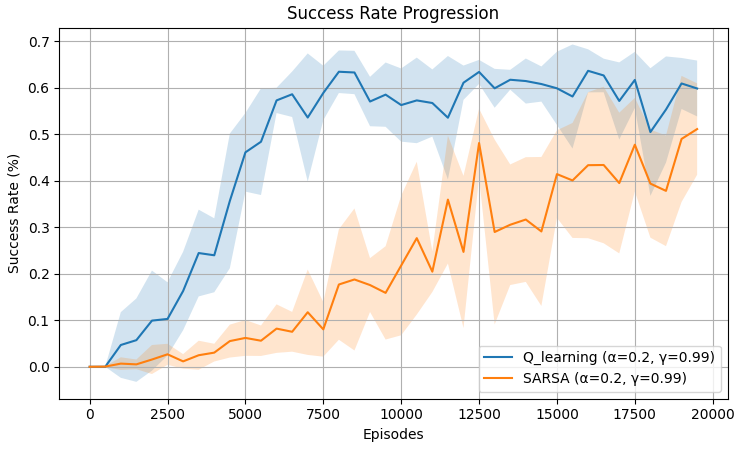
\includegraphics[scale=0.4]{images/comparison_sarsa_Q.png}
    \end{minipage}%
    
\end{block}

\end{frame}

%------------------------------------------------

\section{Simple Multi-agent Reinforcement Learning (MARL) setup}

\begin{frame}[plain]
    \vspace{0.15\textheight}
    \begin{center}
        {\bfseries Section \thesection} 
        
        \vspace{0.5cm} 
        
        {\Large\bfseries\insertsectionhead} 
    \end{center}
\end{frame}

%------------------------------------------------
\begin{frame}{Introducing Multi-Agent RL (MARL)}

\textbf{Game Types:} \\
\framebox{Cooperative (shared reward)}, competitive, or mixed

\vspace{1em}

\begin{minipage}[T]{0.6\textwidth}
    \vspace{-10pt}
    \href{https://github.com/edabier/MARL-project/blob/main/game_gif/centralized-2-agent-coop.gif}{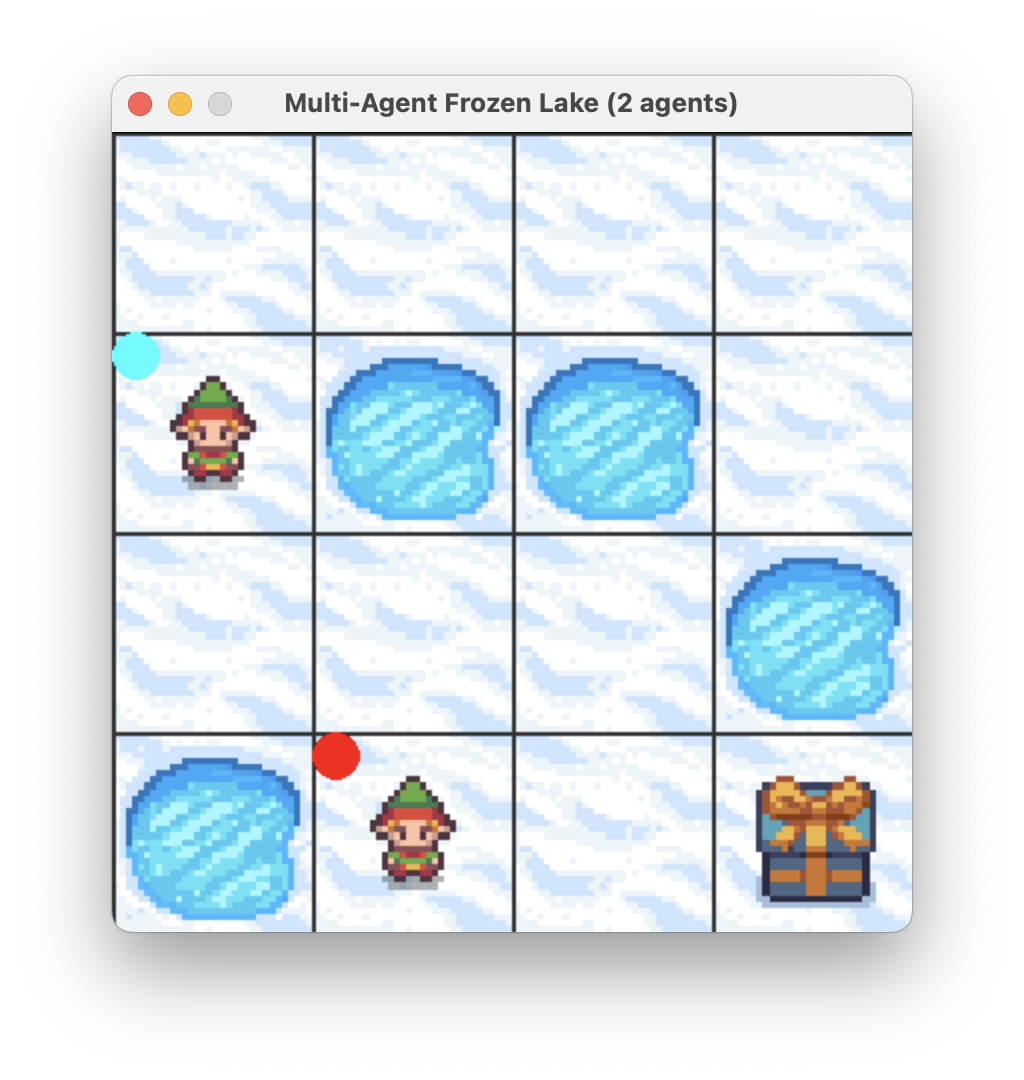
\includegraphics[height=6.7cm]{images/multi-agent.png}}
\end{minipage}
\hspace{-50pt}
\begin{minipage}[T]{0.5\textwidth}
    \vspace{-100pt} % Force top alignment
    \begin{block}{Max reward:} \\
    Agents arrive \textbf{together}: \textit{favors cooperation}
    \end{block}
\end{minipage}

\end{frame}

%------------------------------------------------

\begin{frame}{How to handle multi agents?}

\begin{block}{\textbf{Value iteration}}
    We can simply apply the same value iteration as in single agent setup to learn the \textbf{optimal} policy.
\end{block}

\begin{block}{Reducing to single agent}
   Naive and intuitive approach: reduce to a single agent approach, and for that we have two options: 

   \begin{itemize}
       \item \underline{Centralized Q-Learning (CQL)}: Train a single \textbf{central policy} receiving all agents’ observations and selects actions for each agents.
       \item \underline{Independant Q-Learning (IQL)}: Every agent learns its \textbf{own policy}, based on its observations, state, actions and history, ignoring the other agents.
   \end{itemize}
\end{block}

\end{frame}

%------------------------------------------------

\begin{frame}{Value iteration}
    \begin{center}
        \scriptsize
        \begin{minipage}{0.85\textwidth} 
            \begin{block}{Pseudo code}
                \begin{algorithm}[H]
                    \DontPrintSemicolon
                    
                    \KwOutput{Initialize $V_i^\pi(s)$ for each agent i and each state s (e.g., $V_i^\pi(s) = 0$  $\forall$  $s, i$)}
                    
                    Repeat until convergence:
                    
                    \For{each agent i and each state s }{
                        $V_i(s) = \displaystyle \max_{a_i} \sum P(s' | s, a_1, a_2, ..., a_n) * [R(s, a_1, a_2, ..., a_n, s') + \gamma * V_i(s')] $
                    }
                    \Return $\pi_i^\star(s) = \displaystyle arg\max_{a} P(s' | s, a_1, a_2, ..., a_n) * [R_i(s, a_1, a_2, ..., a_n, s') + \gamma * V_i(s')]$
                \end{algorithm} 
            \end{block}
        \end{minipage}
    \end{center}
    
    \begin{columns} 
        \begin{column}{0.4\textwidth}
            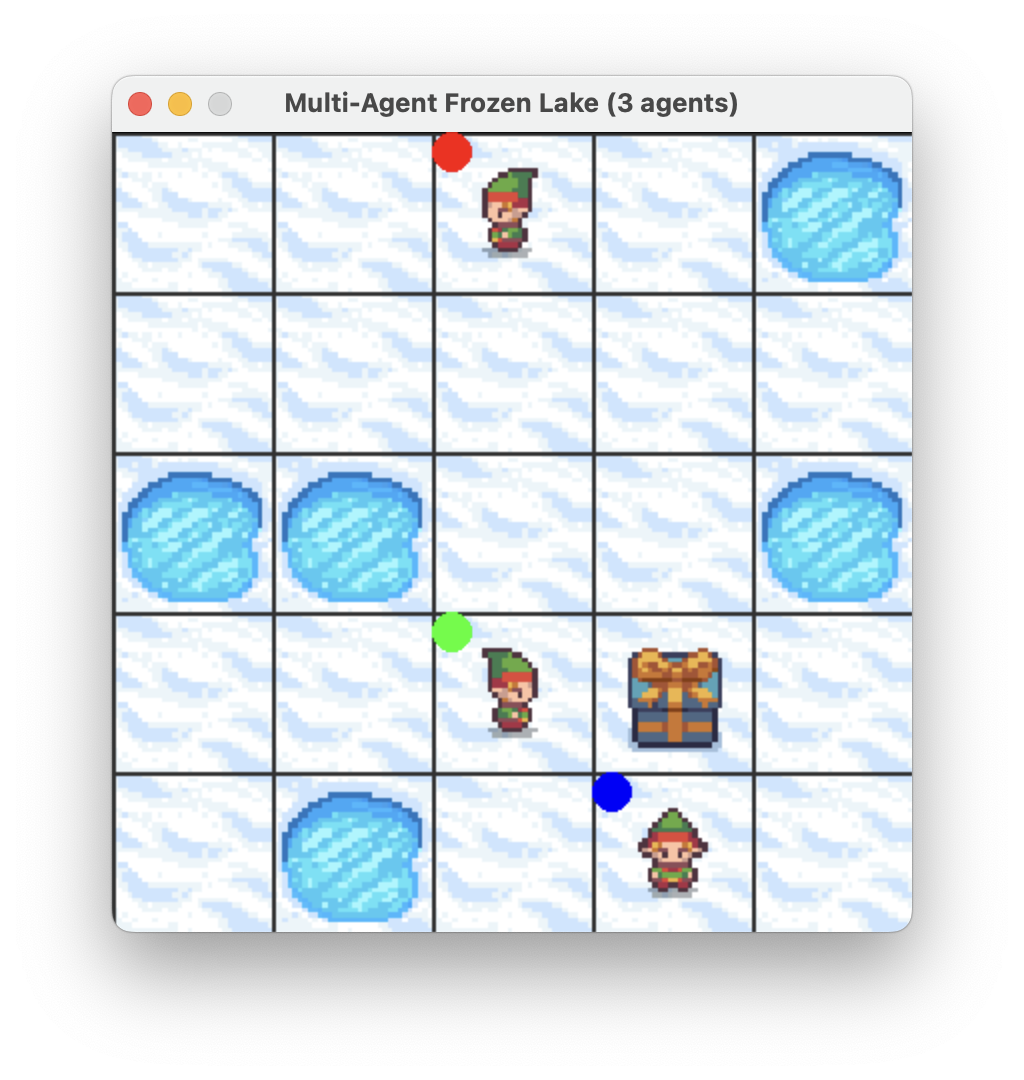
\includegraphics[scale=0.2]{images/5x5-ma.png}
        \end{column}
        \hspace{-50pt}
        \begin{column}{0.6\textwidth}
            \vspace{-20pt}
            \begin{alertblock}{limitations}
                Double \mintinline{python}{ for} loop: (agents + states) $\to$ can become very heavy.  
                \textbf{For example}, a $5\times5$ FrozenLake grid (25 positions) with 3 players, with 4 actions each = $(25 \times 4)^3 = 10e^6$ iterations, repeated \textit{n} times until convergence!
            \end{alertblock}
        \end{column}
    \end{columns}
\end{frame}

%------------------------------------------------

\begin{frame}{Central Q-Learning}
    We \textbf{aggregate} all agents' states, observations and actions and we want to learn a central policy selecting every action in the \textbf{joint-action space} $A = A_0 \times A_1 \times ... \times A_N$ for N agents.

    \begin{figure}[h!]
        \centering
        \begin{minipage}{0.45\textwidth} 
            \centering
            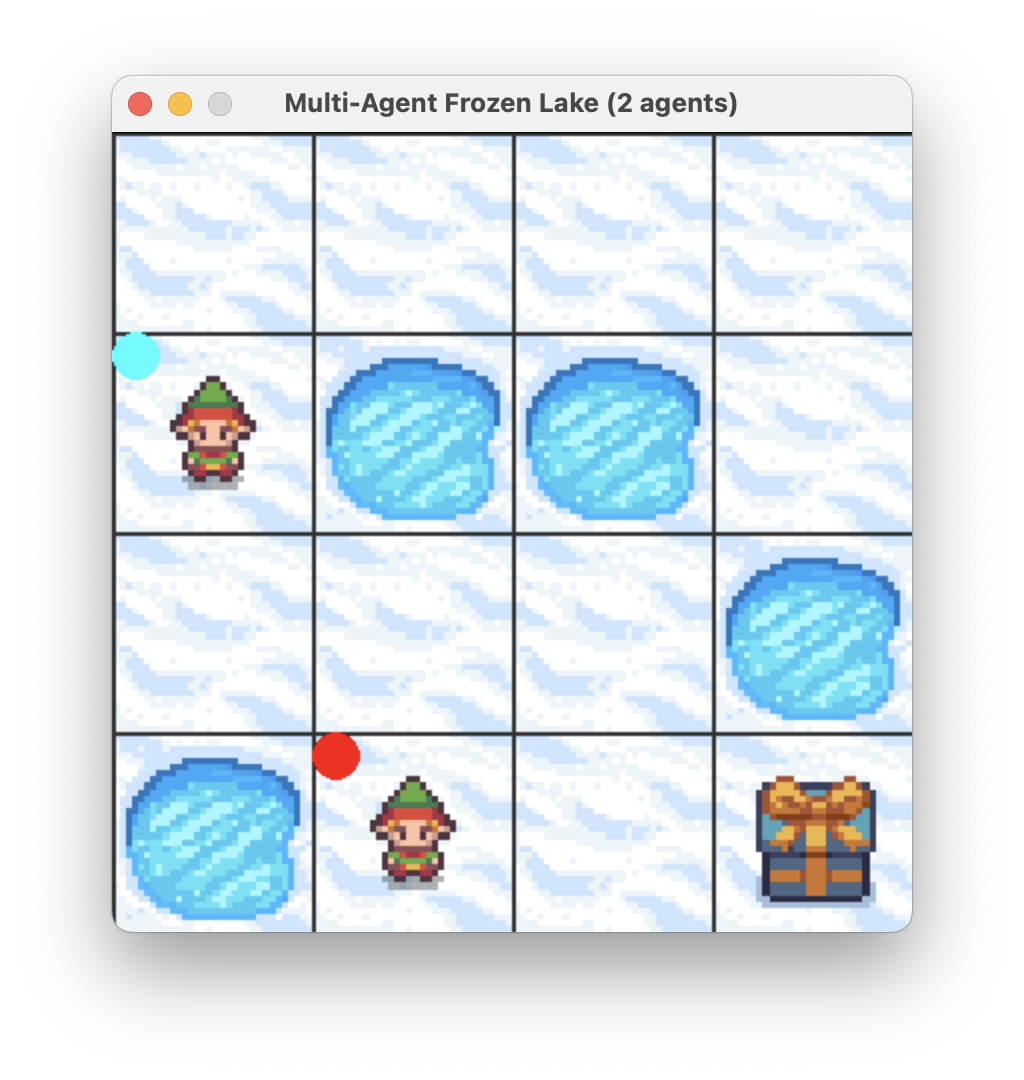
\includegraphics[scale=0.3]{images/multi-agent.png}
        \end{minipage}%
        \begin{minipage}{0.45\textwidth} 
            \begin{alertblock}{Limitations}
            \underline{Curse of dimensionality}: the size of the joint action space grows exponentially with \textbf{n} (the number of agents): $A = A_i^n$
            \end{alertblock}
        \end{minipage}
    \end{figure}

\end{frame}

%------------------------------------------------

\begin{frame}{Central Q-Learning - curse of dimensionality}
    
\centering
\begin{columns}
    \begin{column}{0.5\textwidth}
        \begin{block}{2 agents - $4 \times 4$ grid}
        \scriptsize
            \centering
            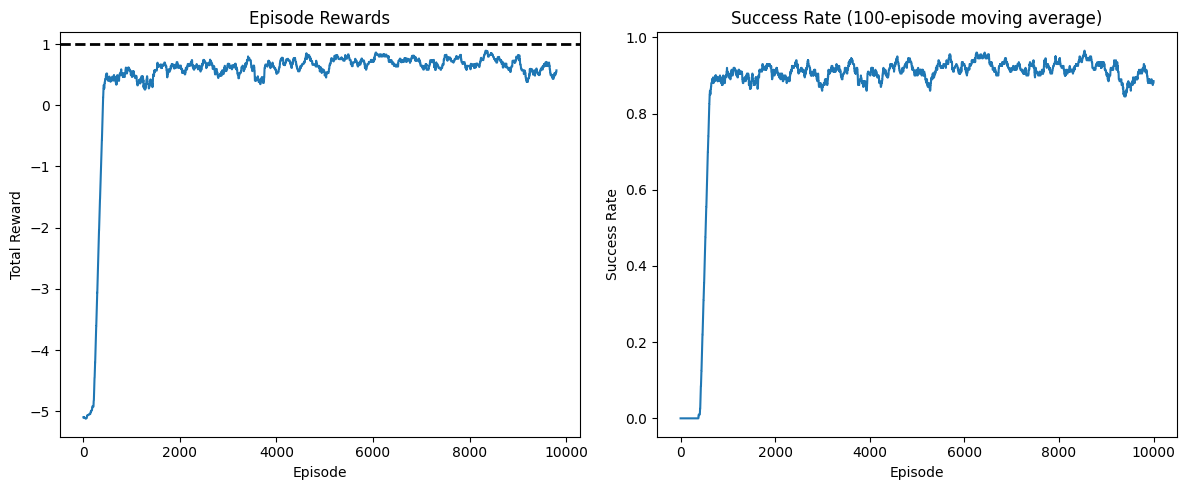
\includegraphics[scale=0.18]{images/2-agents-4x4-10000ep.png}
            
            $10e4$ episodes, \colorbox{lightgreen}{converged} in \textbf{0.9s}
        \end{block}
    \end{column}
    \begin{column}{0.5\textwidth}
        \begin{block}{2 agents - $8 \times 8$ grid}
        \scriptsize
            \centering
            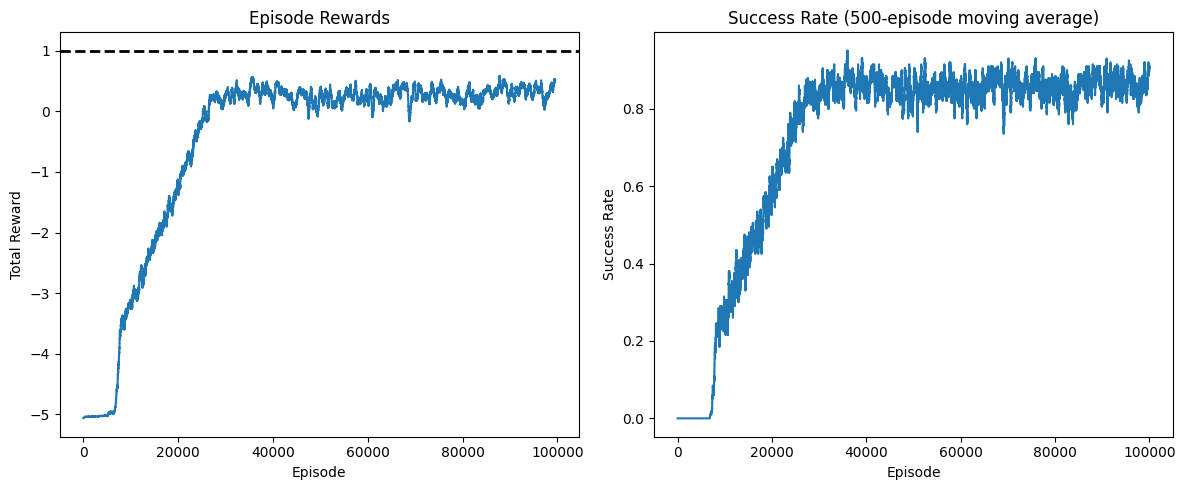
\includegraphics[scale=0.18]{images/2-agents-8x8-100000ep.png}
            
            $10e^5$ episodes, \colorbox{lightgreen}{converged} in \textbf{21.9s}
        \end{block}
    \end{column}
\end{columns}

\begin{columns}
    \begin{column}{0.5\textwidth}
    \scriptsize
        \begin{block}{4 agents - $4 \times 4$ grid}
            \centering
            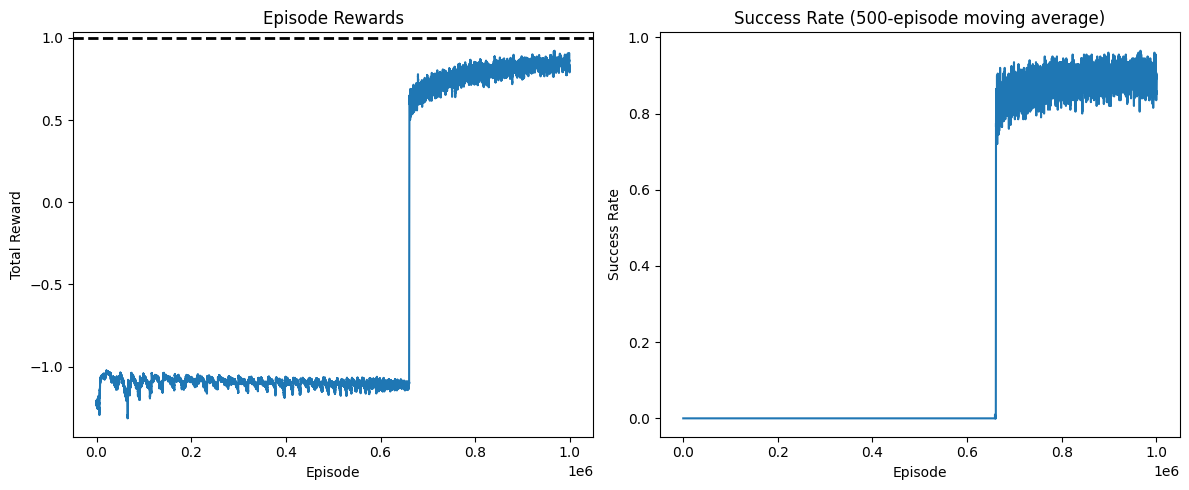
\includegraphics[scale=0.18]{images/4-agents-4x4-10e6.png}
            
            $10e^6$ episodes, \colorbox{lightgreen}{converged} in \textbf{2mn5s}
        \end{block}
    \end{column}
    \begin{column}{0.5\textwidth}
    \scriptsize
        \begin{block}{4 agents - $6 \times 6$ grid}
            \centering
            \sethlcolor{lightred}
            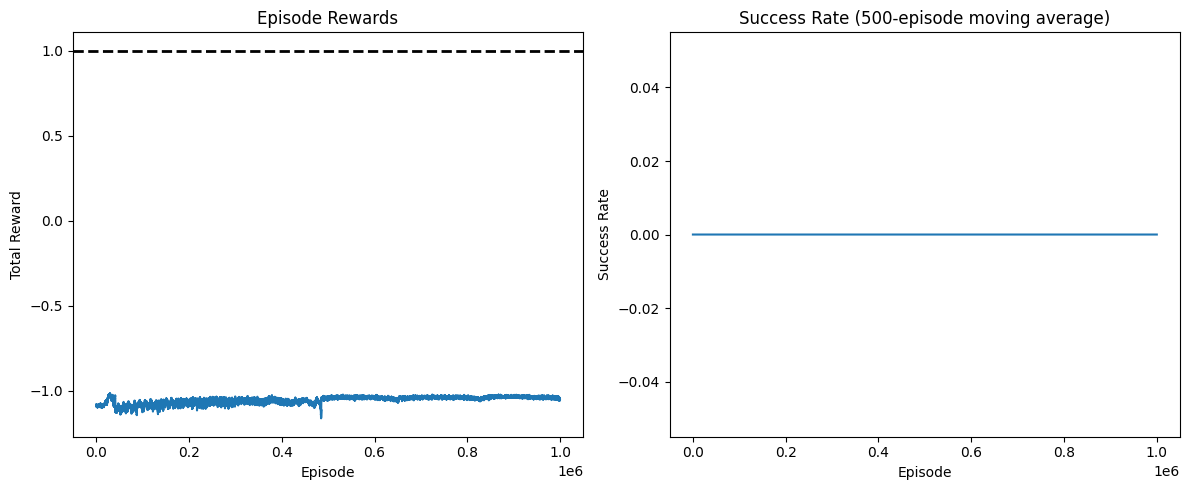
\includegraphics[scale=0.18]{images/4-agents-6x6-10e6.png}
            
            $10e^6$ episodes, \colorbox{lightred}{did not converge} after \textbf{2mn26s}
        \end{block}
    \end{column}
\end{columns}


\end{frame}

%------------------------------------------------

\begin{frame}{Central Q-Learning - curse of dimensionality}

\center
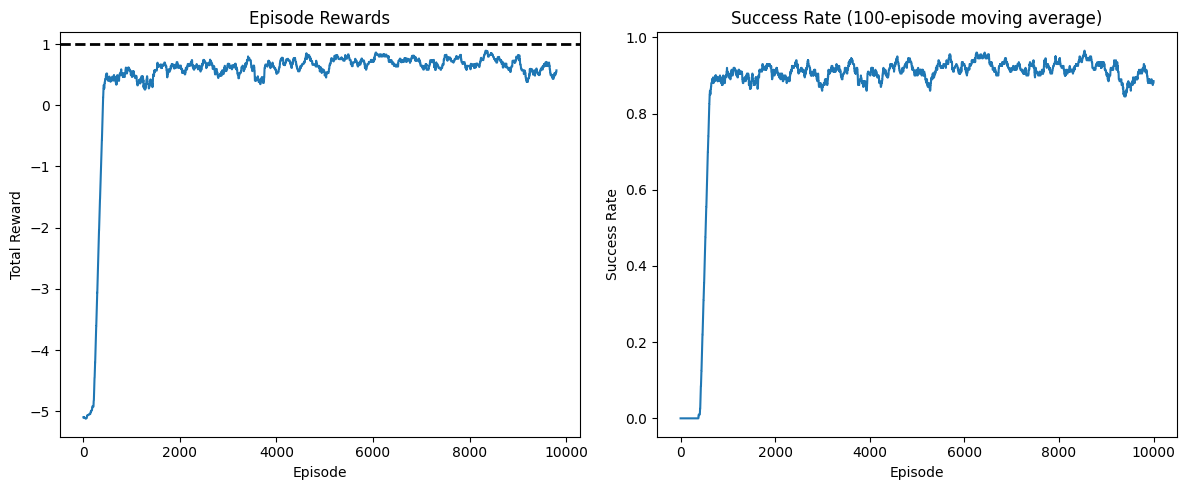
\includegraphics[scale=0.4]{images/2-agents-4x4-10000ep.png}

\begin{minipage}{0.4\textwidth}
    \begin{block}{\center 2 agents - $4 \times 4$ grid} 
            \center
            \vspace{-10pt}
            \begin{inparaitem}
                \item \textbf{n\_episodes = $10e^4$}
                \item \textbf{\colorbox{lightgreen}{converged} in \textbf{0.9s}}
            \end{inparaitem}  
    \end{block}
\end{minipage}

\end{frame}

%------------------------------------------------

\begin{frame}{Central Q-Learning - curse of dimensionality}

\center
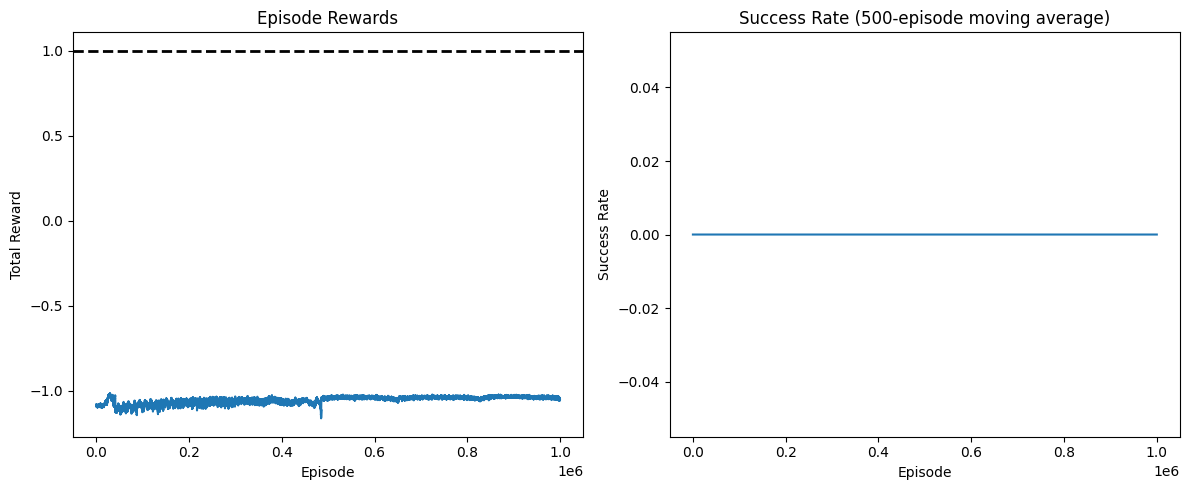
\includegraphics[scale=0.4]{images/4-agents-6x6-10e6.png}

\begin{minipage}{0.5\textwidth}
    \begin{block}{\center 4 agents - $6 \times 6$ grid} 
            \center
            \vspace{-10pt}
            \begin{inparaitem}
                \item \textbf{n\_episodes = $10e^6$}
                \item \textbf{\colorbox{lightred}{did not converge} after \textbf{2mn26s}}
            \end{inparaitem}  
    \end{block}
\end{minipage}

\end{frame}

%------------------------------------------------

\begin{frame}{A new setup}

    \begin{figure}[h!]
        \centering
        \begin{minipage}{0.3\textwidth} 
            \centering
            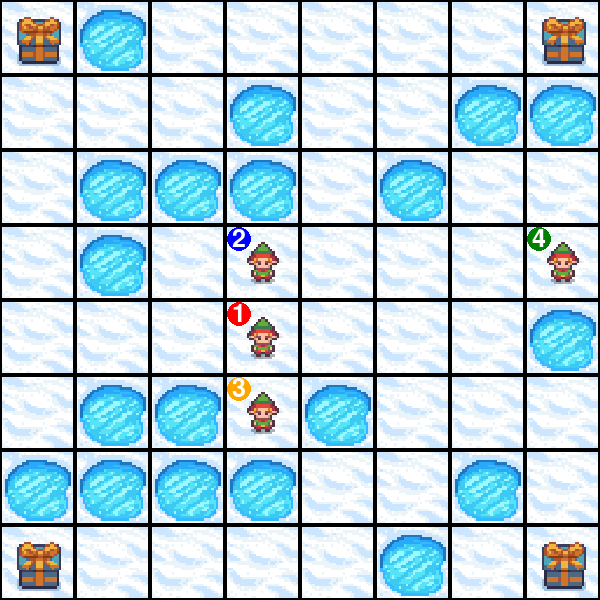
\includegraphics[scale=0.2]{images/step_000.png}
            \caption{Reward = \textbf{0}}
        \end{minipage}%
        \hspace{10pt}
        \begin{minipage}{0.3\textwidth} 
            \centering
            \href{https://raw.githubusercontent.com/edabier/MARL-project/main/game_gif/frozen4winGIF.gif}{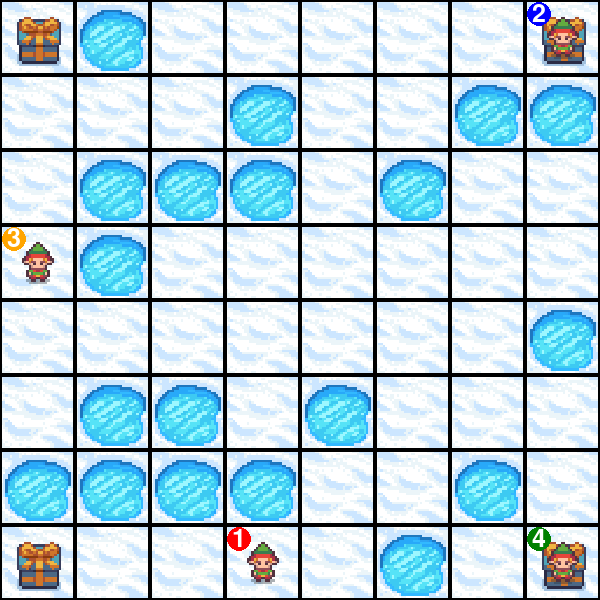
\includegraphics[scale=0.2]{images/step_007.png}}
            \caption{Reward = \textbf{+200}}
        \end{minipage}%
        \hspace{10pt}
        \begin{minipage}{0.3\textwidth} 
            \centering
            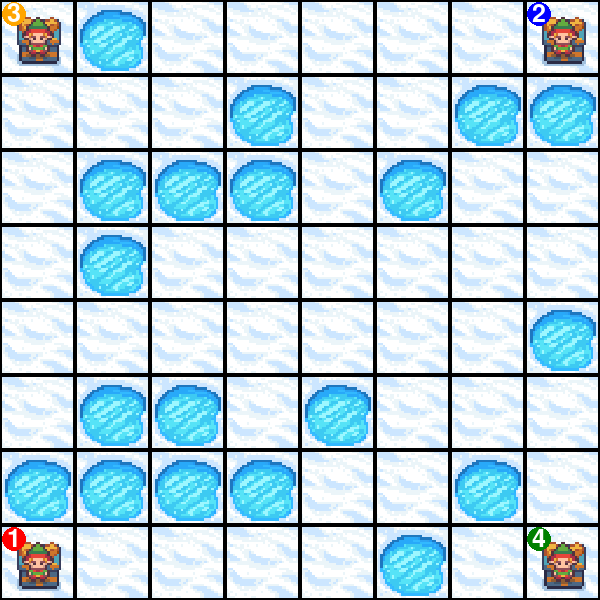
\includegraphics[scale=0.2]{images/step_010.png}
            \caption{Reward = \textbf{+400}}
        \end{minipage}
    \end{figure}

    Four agents in a FrozenLake setup, each trying to reach a different goal and avoid \textbf{collisions} between agents to maximize their reward.

\end{frame}

%---------------------------------------------

\begin{frame}{Independent Q-Learning}
     
    \begin{block}{Key Idea}
        Each agent learns its policy or value function \emph{independently / as if it were alone.}
        
        \medskip
        Each agent assumes the other agents are part of the \textbf{environment.}

        \medskip
        Total Action space $\boldsymbol{A = \sum_{i=1}^{N} A_i} \neq \prod_{i=1}^{N} A_i$ for Central Q-Learning.
    \end{block}
    
    \begin{minipage}{0.45\textwidth} 
        \begin{alertblock}{Limitations}
            \begin{itemize}
                \item Environment appears \textbf{non-stationary} to each agent (others are learning/changing).
                \item Can lead to instability or slower convergence.
            \end{itemize}
        \end{alertblock}

        \vspace{0.5em}
        {\href{https://raw.githubusercontent.com/edabier/MARL-project/main/game_gif/IQL10AGENT.gif}{\textcolor{blue}{[video]}}}
    \end{minipage}
    \hfill
    \begin{minipage}{0.5\textwidth}
        \centering
        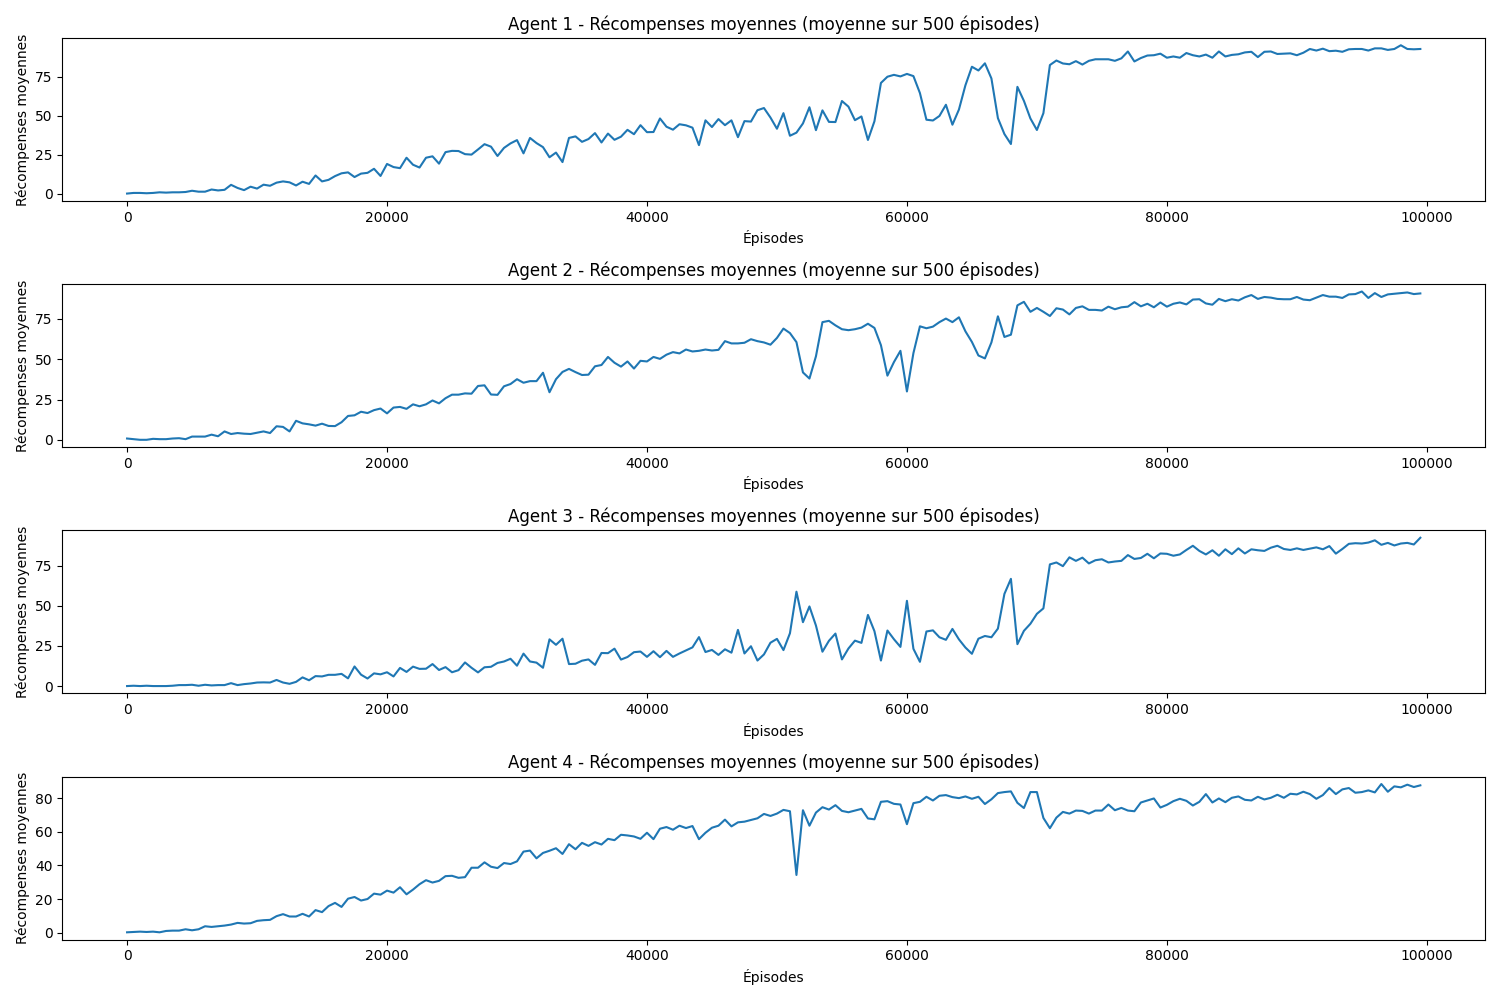
\includegraphics[scale=0.15]{images/AAA.png}
        \captionof{figure}{Fluctuating reward due to non-stationarity.}
    \end{minipage}
    
\end{frame}

%------------------------------------------------

\begin{frame}{Independent Q-Learning}
    \centering
    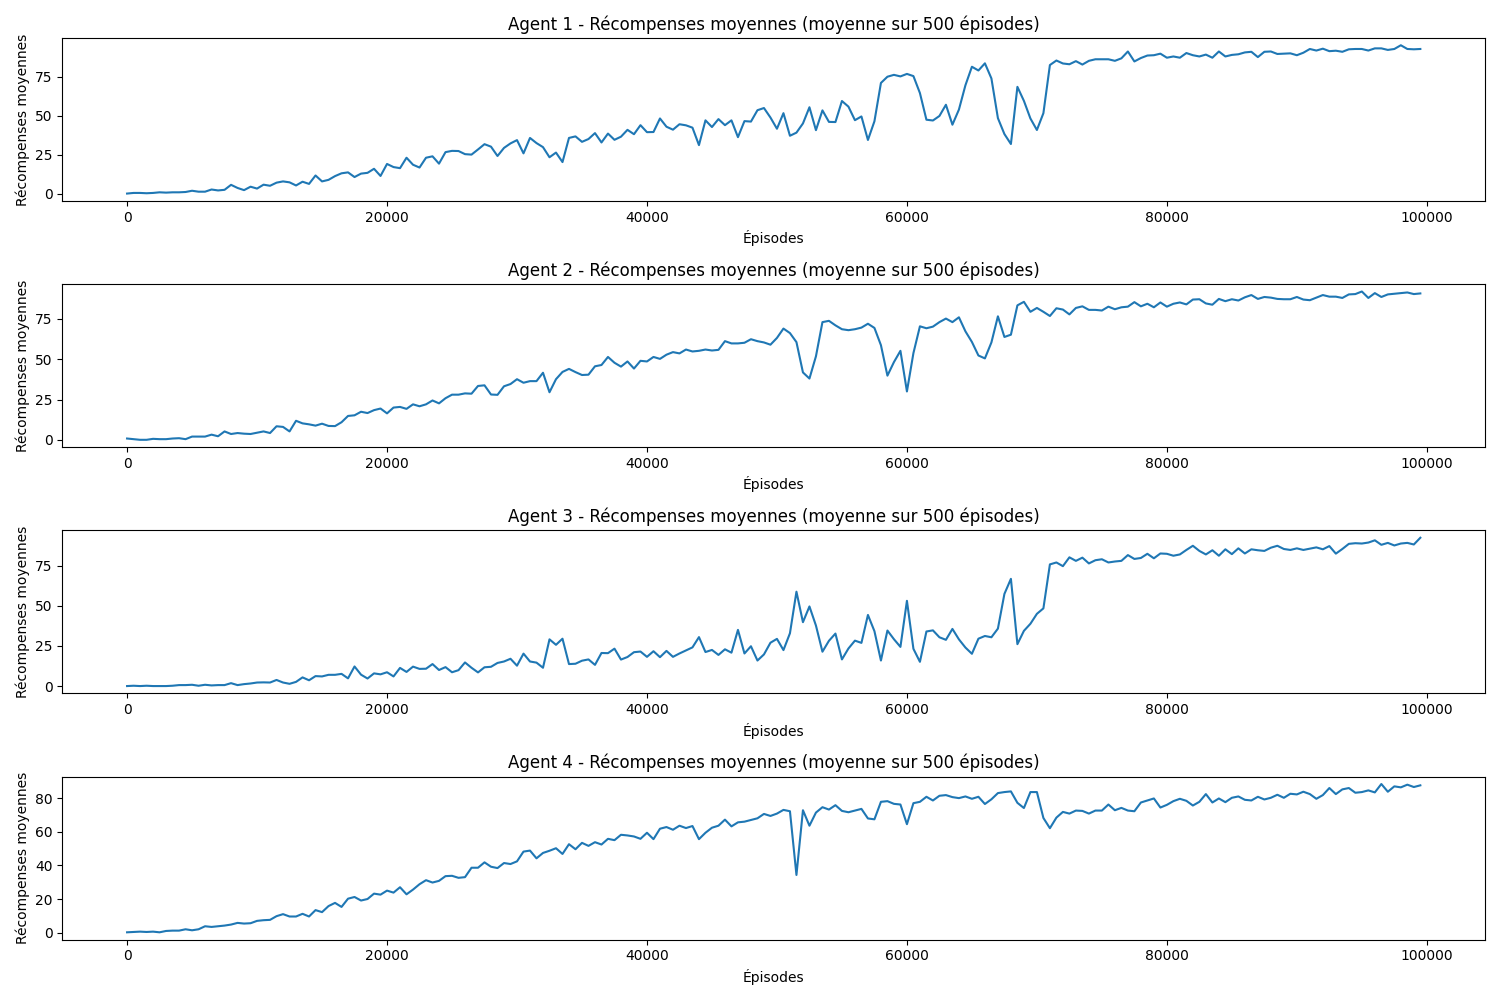
\includegraphics[width=0.9\paperwidth,height=0.75\paperheight,keepaspectratio]{images/AAA.png}
    
    \vspace{1em}
    \captionof{Figure: }{Fluctuating reward due to non-stationarity.}
\end{frame}

%------------------------------------------------

\begin{frame}{Alternating Independent Q-Learning}

    \begin{columns}[T] % align all columns to top
        % Left column
        \column{0.4\textwidth}
        \begin{block}{Key Idea}
            Each agent learns \emph{independently / as if it were alone}, but takes turns learning.  
            This helps reduce non-stationarity by stabilizing each agent’s learning process.
        \end{block}

        % Right column
        \column{0.6\textwidth}
        \centering
        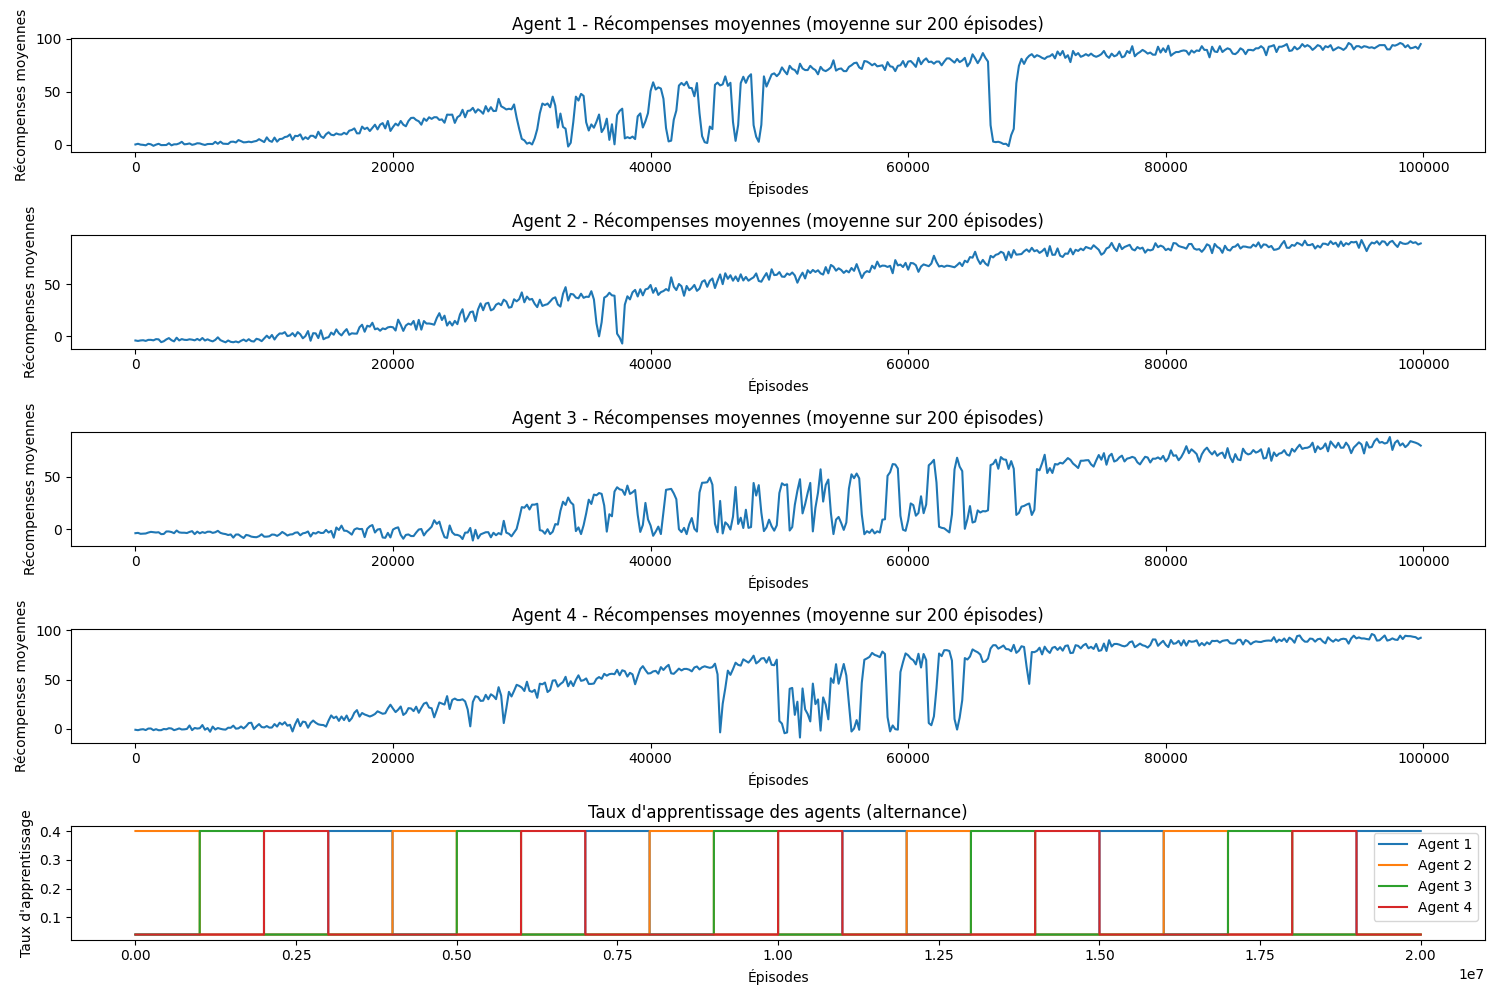
\includegraphics[scale=0.23]{images/alt_learning.png} \\
        {\small Reward of agents with alternating learning rates.}
    \end{columns}

    \vspace{0.5cm}
    \begin{minipage}{0.2\textwidth}
    {\href{https://raw.githubusercontent.com/edabier/MARL-project/main/game_gif/AltIqlwin10.gif}{\textcolor{blue}{[video]}}}
    \end{minipage}
\end{frame}

%------------------------------------------------

\begin{frame}{Alternating Independent Q-Learning}
    \centering
    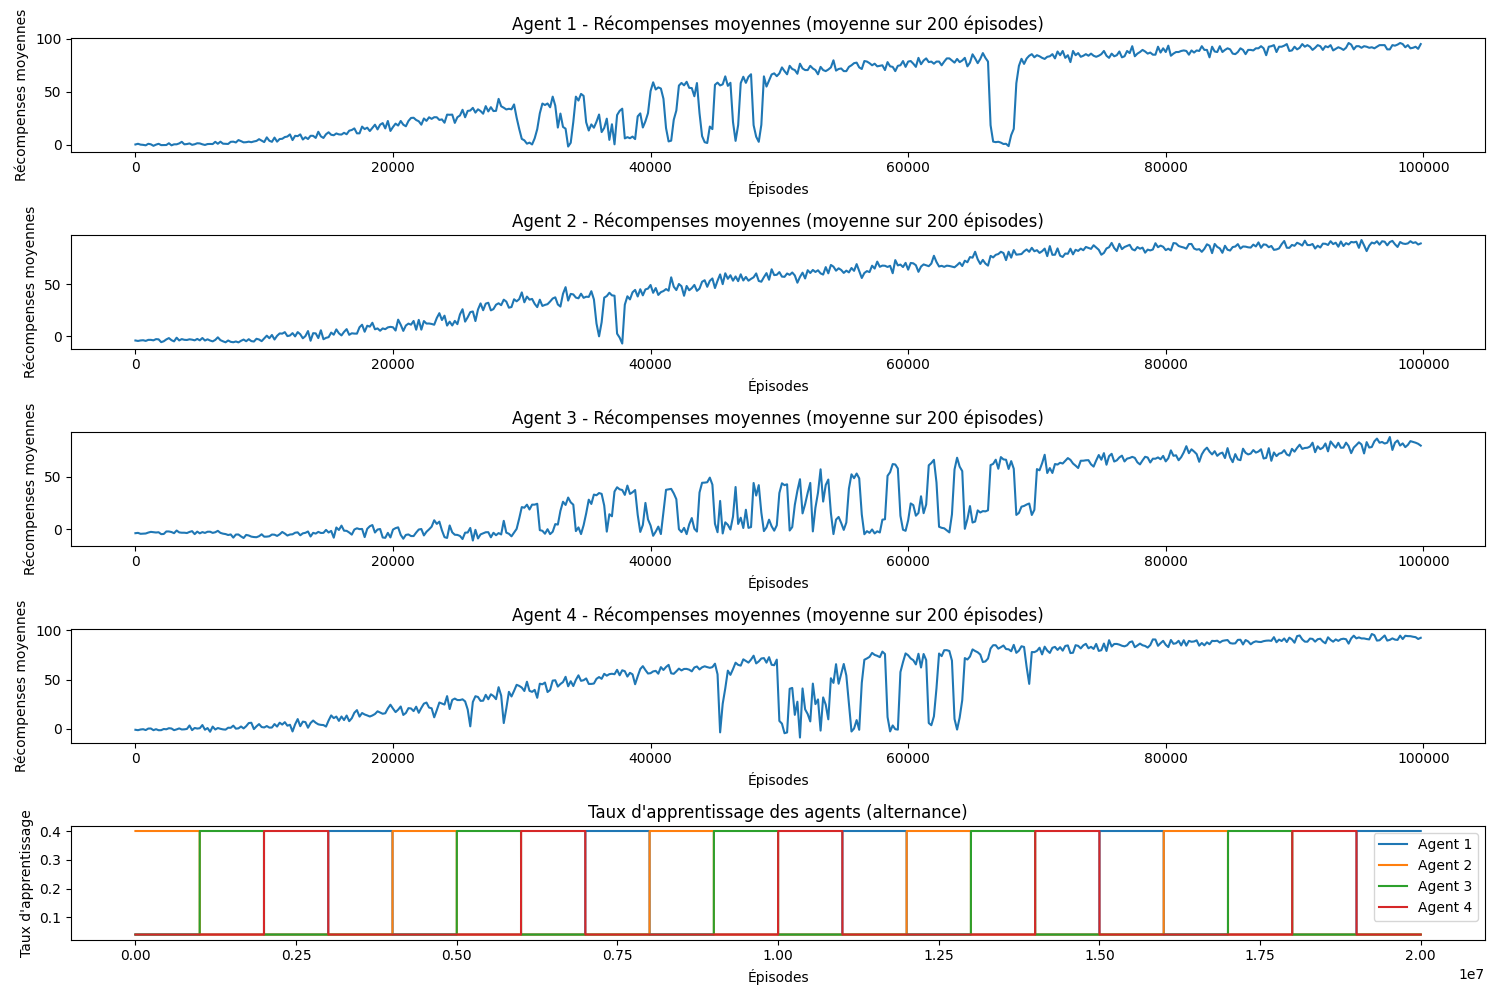
\includegraphics[width=0.9\paperwidth,height=0.75\paperheight,keepaspectratio]{images/alt_learning.png}
    
    \vspace{1em}
    \captionof{Figure: }{Alternating Q learning reward and alternating learning rates }
\end{frame}

%------------------------------------------------

\section{Conclusion and perspectives}

\begin{frame}[plain]
    \vspace{0.15\textheight}
    \begin{center}
        {\bfseries Section \thesection} 
        
        \vspace{0.5cm} 
        
        {\Large\bfseries\insertsectionhead} 
    \end{center}
\end{frame}

%------------------------------------------------

\begin{frame}{What about more complex games?}
\center
    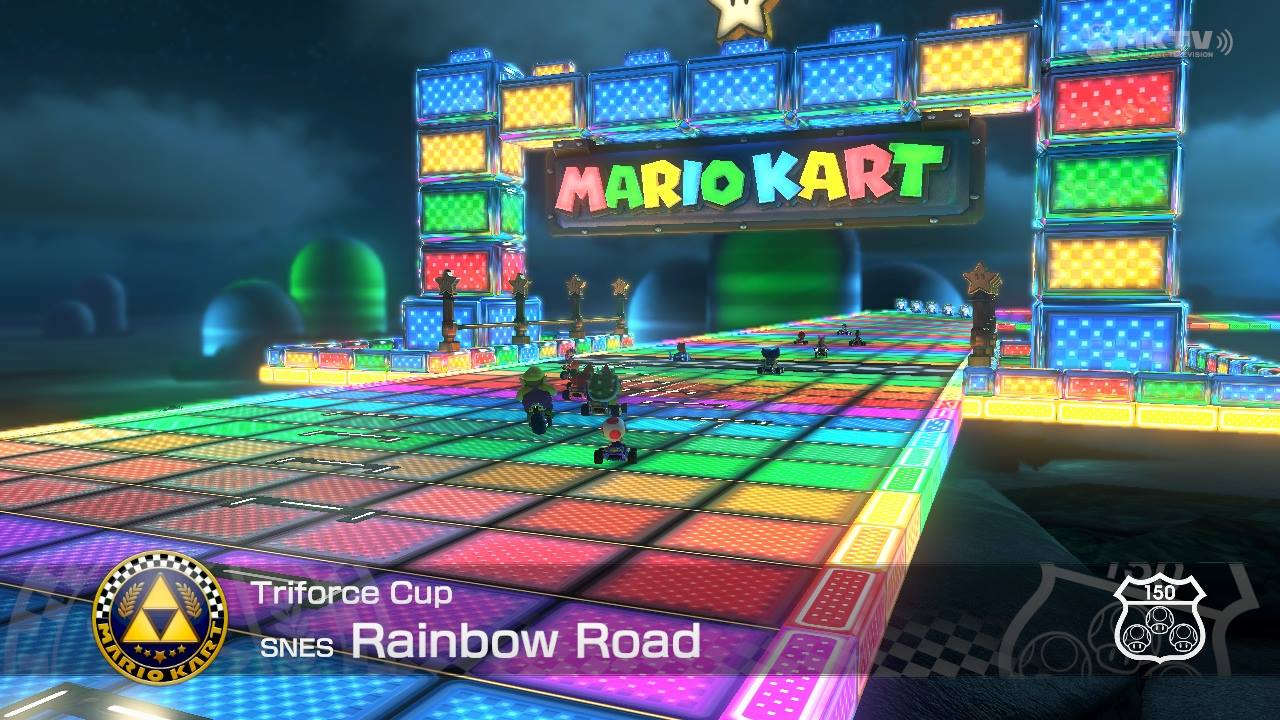
\includegraphics[scale=0.25]{images/mk8snes.jpg}
    
    Classic Q-Learning methods will \colorbox{lightred}{not be sufficient} $\to$ use of \textbf{Deep Learning} through Deep Q-Learning for example.
\end{frame}

% %------------------------------------------------

\begin{frame}{Conclusion}
\begin{block}{\textbf{Reinforcement Learning (RL)}}
     Agents learn by interacting with the environment.
    \begin{itemize}
        \item The agent learns a policy by optimizing one of the \textbf{value function} $V^*(s)\quad or\quad Q^*(s,a) $
    \end{itemize}
\end{block}
\begin{block} {\textbf{Multi-Agent RL (MARL)}}
     Agents must also adapt to each other, increasing complexity.
    \begin{itemize}
    \item \textbf{Central Q learning}  Accurate but not scalable.
    \item \textbf{Independent Q-Learning (IQL)}  Scalable, but suffers from non-stationarity.
    \item \textbf{Alternating learning strategies} Helps improve stability and convergence.
    \item \textbf{Deep learning + Q-function} Enables learning in more complex environments.
    \end{itemize}
\end{block}
\vspace{0.5em}
% \textbf{In short:} MARL is key to building intelligent systems capable of learning in dynamic, multi-agent environments.
\center
    \raisebox{-0.25\height}{
\includegraphics[scale=0.3]{images/github-mark.png}} 
    Come see our work! 
    { \href{https://github.com/edabier/MARL-project}{{\textcolor{blue}{\underline{https://github.com/edabier/MARL-project}}}}}

\end{frame}

%----------------------------------------------------------------------------------------

\end{document}